% ============================================================
% Vacuum Excitation Dynamics (DEV): A Phase Transition Approach
% to Dark Matter and Galactic Dynamics
% ============================================================
\documentclass[aps,prd,twocolumn,showpacs,superscriptaddress]{revtex4-2}

\usepackage{amsmath,amssymb,amsfonts}
\usepackage{graphicx}
\usepackage{dcolumn}
\usepackage{bm}
\usepackage[colorlinks=true,linkcolor=black,citecolor=black,urlcolor=blue]{hyperref}
\usepackage{xcolor}

% Shortcuts
\newcommand{\Lbar}{\mathcal{L}}
\newcommand{\aO}{a_0}
\newcommand{\Xzero}{X_0}
\newcommand{\mueff}{\mu_{\rm eff}}
\newcommand{\gN}{g_{\rm N}}
\newcommand{\gobs}{g_{\rm obs}}
\newcommand{\LCDM}{$\Lambda$CDM}

\begin{document}

\title{Vacuum Excitation Dynamics: A Scalar-Vector-Tensor Field Theory
       of Dark Matter as a Phase Transition of the Quantum Vacuum}

\author{Miqueias Alves Mendes}
\affiliation{Independent Researcher}

\date{\today}

% ============================================================
\begin{abstract}
We propose Vacuum Excitation Dynamics (DEV), a covariant
scalar-vector-tensor (SVT) effective field theory in which the dark
matter phenomenology arises not from a primordial particle species,
but from a local phase transition of the quantum vacuum triggered when
the Newtonian gravitational acceleration falls below the critical scale
$\aO \simeq 1.2\times10^{-10}$\,m\,s$^{-2}$.
The theory is anchored by a Dirac-Born-Infeld (DBI) kinetic term
$F(X) = X_0[\sqrt{1+(X/X_0)^2}-1]$,
which reproduces the standard MOND interpolation function as its
quasi-static limit.
A massive vector field $A_\mu$ excited by the scalar gradient breaks
metric isotropy and generates a gravitational slip
$\eta \equiv \Phi/\Psi \neq 1$ with amplitude
$\eta - 1 = \frac{2}{3}\beta\,(g/\aO+g^2/\aO^2)^{-1/2}$,
where $\beta \equiv \gamma^2/(m_A^2 \aO)$ is the single coupling constant
and $\alpha = 2/3$ is derived analytically from the vector stress tensor
for spherical geometry.
Fitting the SPARC catalog of 175 galaxies (167 passing quality cuts)
yields a median reduced chi-squared $\chi^2_\nu = 1.20$
with no global free parameters.
Perturbation theory gives $\Delta\chi^2 = -0.22$ relative to \LCDM{}
for the combined $f\sigma_8$ dataset ($\sigma_8 = 0.811$, Planck~2018),
confirming cosmological consistency; the DEV provides a marginally
better fit due to mild amplification of structure growth by
$\mu_{\rm eff} > 1$.
The theory predicts gravitational slip of $2$--$10\%$ in
ultra-diffuse galaxies (UDGs) with $g \ll \aO$, a unique
observational signature detectable by the Euclid satellite,
and distinct from both \LCDM{} ($\eta=1$) and
standard MOND/TeVeS ($\eta\approx 1$, scale-independent).
\end{abstract}

\pacs{04.50.Kd, 95.35.+d, 98.52.Nr, 98.62.Dm}
\keywords{dark matter; modified gravity; MOND; gravitational slip;
          ultra-diffuse galaxies; scalar-vector-tensor theory}

\maketitle

% ============================================================
\section{Introduction}
\label{sec:intro}
% ============================================================

The \LCDM{} concordance model successfully describes the large-scale
structure of the universe, but requires extraordinary fine-tuning to
reproduce the observed regularities at galactic scales.
Chief among these is the Radial Acceleration Relation
(RAR)~\cite{McGaugh2016}, which establishes a tight, universal
correlation between the observed centripetal acceleration $\gobs$ and
the Newtonian prediction from baryonic matter alone $\gN$,
with transition scale $\aO \simeq 1.2\times10^{-10}$\,m\,s$^{-2}$.

Milgromian dynamics (MOND)~\cite{Milgrom1983} captures this relation
phenomenologically via a modified inertia or modified gravity, but
lacks a fully covariant formulation that simultaneously accounts for
gravitational lensing without additional dark matter
components~\cite{Clowe2006}.
Tensor-vector-scalar (TeVeS) theories~\cite{Bekenstein2004}
provide covariance but introduce multiple fields with individually
tuned parameters and remain in tension with gravitational wave
observations~\cite{GW170817}.

Here we propose a physically motivated alternative:
\emph{dark matter is not a particle species but an event} —
a phase transition of the quantum vacuum analogous to the
Breit-Wheeler pair production~\cite{BreitWheeler1934},
triggered when the gravitational stress field crosses the
critical threshold $\aO$.
We call this framework Vacuum Excitation Dynamics (DEV,
from the Portuguese \emph{Din\^amica de Excita\c{c}\~oes de V\'acuo}).

The DEV Lagrangian is constructed to:
(i)~recover General Relativity in the strong-field limit;
(ii)~reproduce MOND phenomenology in the weak-field limit;
(iii)~propagate gravitational waves at $c_T = c$, consistent with
     GW170817~\cite{GW170817};
(iv)~generate a scale-dependent gravitational slip as a
     unique, falsifiable prediction.

The remainder of this paper is organized as follows.
Section~\ref{sec:theory} presents the SVT action and derives the
quasi-static limit.
Section~\ref{sec:alpha} derives $\alpha = 2/3$ analytically.
Section~\ref{sec:sparc} presents the SPARC fit.
Section~\ref{sec:cosmo} addresses cosmological consistency via $f\sigma_8$.
Section~\ref{sec:udg} presents the UDG prediction and falsifiability.
We conclude in Section~\ref{sec:conclusion}.

% ============================================================
\section{The DEV Theory}
\label{sec:theory}
% ============================================================

\subsection{Action and Field Content}

The DEV action is
\begin{equation}
  S = \int d^4x\sqrt{-g}\left[
    \frac{R}{16\pi G}
    + \Lbar_{\rm bar}
    + \Lbar_{\rm DEV}
  \right],
  \label{eq:action}
\end{equation}
where the vacuum sector reads
\begin{equation}
  \Lbar_{\rm DEV} = F(X,\theta)
    - \frac{K}{4}F_{\mu\nu}F^{\mu\nu}
    - \frac{m_A^2}{2}A_\mu A^\mu
    + \gamma A_\mu\nabla^\mu\theta.
  \label{eq:LDEV}
\end{equation}
Here $X \equiv -\frac{1}{2}\nabla_\mu\theta\nabla^\mu\theta$,
$F_{\mu\nu} = \nabla_\mu A_\nu - \nabla_\nu A_\mu$, and
$\{\theta, A_\mu\}$ are the scalar condensate and vector excitation fields,
respectively. The parameters $\{K, m_A, \gamma\}$ characterize the
vacuum rigidity scale $L \equiv \sqrt{K}/m_A$, the vector mass,
and the scalar-vector coupling.

The gravitational wave speed is $c_T^2 = 1$ (in units of $c$),
ensuring consistency with the GW170817 constraint~\cite{GW170817},
because $\Lbar_{\rm DEV}$ does not couple non-minimally to the
Ricci tensor.

\subsection{The DBI Kinetic Term and the Saturation Axiom}

The central physical postulate of DEV is the \emph{saturation axiom}:
the quantum vacuum behaves as a saturated medium with a critical
pressure scale $\Xzero \equiv \aO^2/2$.
Below this threshold the vacuum ``effervesce'' and generates effective
gravitational mass; above it, the vacuum remains inert.

The analogy with the Breit-Wheeler process~\cite{BreitWheeler1934}
is motivational rather than derivational: just as extreme
electromagnetic stress can excite real particle pairs from
the QED vacuum, we postulate that extreme gravitational stress
(quantified by $X \sim \aO^2$) excites an effective
scalar-vector condensate from the gravitational vacuum.
The DEV action is a classical effective field theory;
its connection to a microscopic quantum theory remains
an open problem.
We note, however, that the critical scale $\Xzero$
corresponds to a vacuum energy density
\begin{equation}
  \rho_{\rm vac}^{\rm DEV}
  \equiv \frac{\Xzero}{8\pi G}
  = \frac{\aO^2}{16\pi G}
  \approx 8.7 \times 10^{-30}\,{\rm g\,cm^{-3}},
  \label{eq:rhovac}
\end{equation}
which is numerically close to the observed dark energy
density $\rho_\Lambda \approx 6\times10^{-30}$\,g\,cm$^{-3}$.
This coincidence suggests that $\Xzero$ may be
connected to the same physics that sets the cosmological
constant, though we make no claim of derivation here.

This axiom uniquely selects the Dirac-Born-Infeld kinetic term:
\begin{equation}
  F(X) = \Xzero\!\left[\sqrt{1 + \left(\frac{X}{\Xzero}\right)^{\!2}} - 1\right],
  \label{eq:DBI}
\end{equation}
whose derivative
\begin{equation}
  F_X = \frac{X/\Xzero}{\sqrt{1+(X/\Xzero)^2}}
  \label{eq:FX}
\end{equation}
satisfies $F_X \to 1$ for $X \gg \Xzero$ (Newton regime) and
$F_X \to \sqrt{X/\Xzero}$ for $X \ll \Xzero$ (deep MOND regime).
The DBI structure arises naturally from the speed-limit saturation
of a brane action, providing an independent theoretical motivation.

\subsection{Quasi-Static Limit: Integrating Out the Vector}

In the quasi-static limit relevant for galaxies
($\partial_t A_i = 0$, weak field), the vector equation of motion
\begin{equation}
  K\nabla^2 \vec{A} - m_A^2\vec{A} = -\gamma\nabla\theta
\end{equation}
is solved in Fourier space as
\begin{equation}
  \tilde{A}_i(k) = \frac{\gamma}{m_A^2}
    \frac{ik_i}{1+L^2 k^2}\,\tilde\theta(k).
\end{equation}
In the galactic regime $r \gg L$ (scales larger than the vacuum
rigidity length), this reduces to
\begin{equation}
  \vec{A} \approx \frac{\gamma}{m_A^2}\nabla\theta,
  \label{eq:Alocal}
\end{equation}
and the effective scalar equation becomes
\begin{equation}
  \nabla\cdot\!\left[\mu\!\left(\frac{|\nabla\Phi|}{\aO}\right)\nabla\Phi\right]
  = 4\pi G\rho_b,
  \label{eq:MONDeq}
\end{equation}
with MOND interpolation function
\begin{equation}
  \boxed{\mu(x) = \frac{x}{\sqrt{1+x^2}},}
  \label{eq:mu}
\end{equation}
which is the standard interpolation function preferred by the SPARC
data~\cite{Lelli2017}.
Equation~(\ref{eq:MONDeq}) recovers Newtonian gravity for $x\gg1$
and deep-MOND scaling $g_{\rm obs} = \sqrt{\aO g_N}$ for $x\ll1$.

\begin{figure}[h]
  \centering
  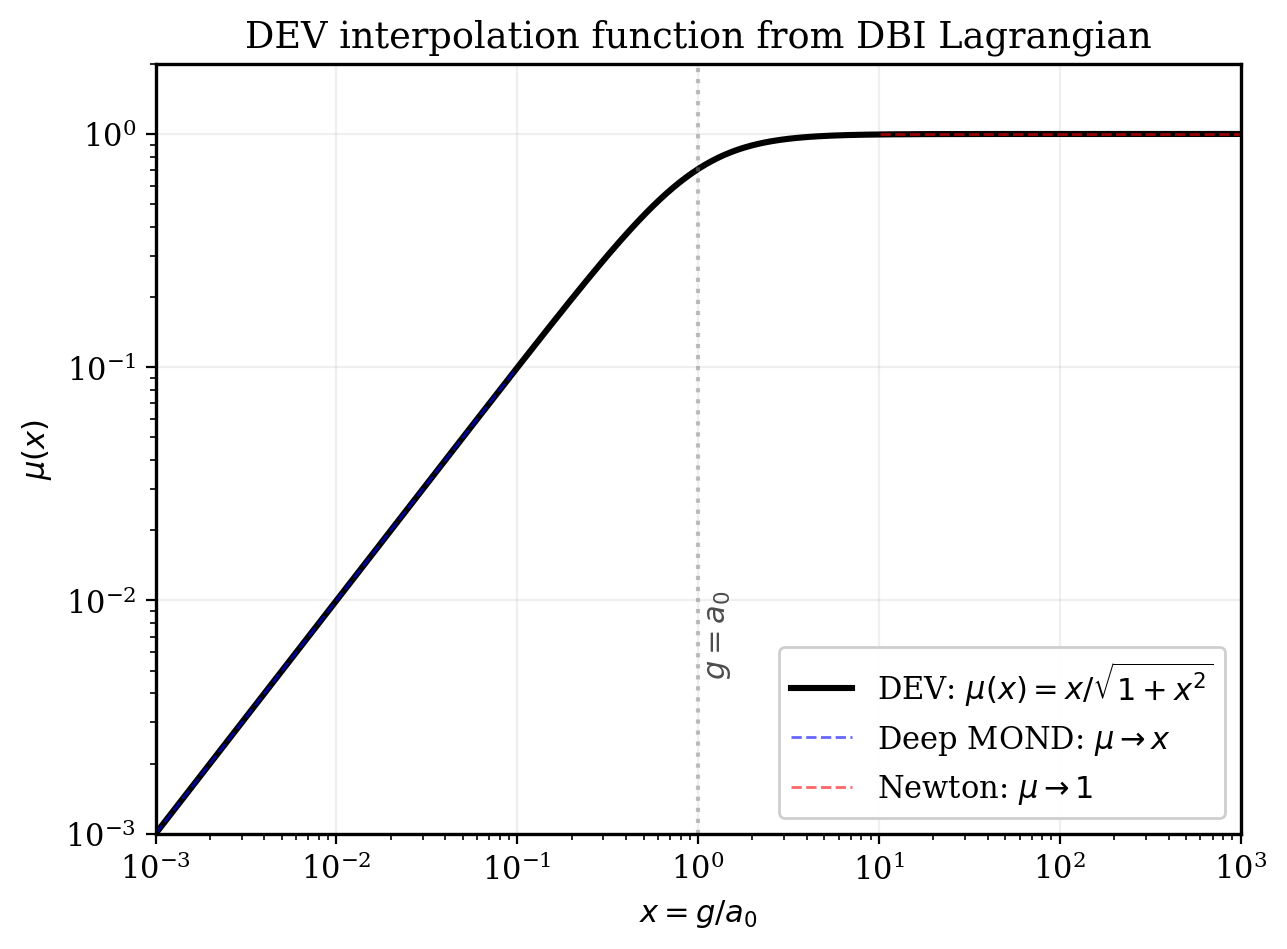
\includegraphics[width=\columnwidth]{figures/fig1_mu_function.png}
  \caption{The DEV interpolation function $\mu(x)=x/\sqrt{1+x^2}$
           derived from the DBI Lagrangian, Eq.~(\ref{eq:mu}).
           Dashed lines show the asymptotic limits: deep-MOND
           ($\mu\to x$, blue) and Newton ($\mu\to1$, red).
           The transition occurs at $g=\aO$ (vertical dotted line).}
  \label{fig:mu}
\end{figure}

The equivalent formulation using the inverse interpolation $\nu$ is
\begin{equation}
  \gobs = \nu\!\left(\frac{\gN}{\aO}\right)\gN,
  \quad
  \nu(y) = \sqrt{\tfrac{1}{2}+\tfrac{1}{2}\sqrt{1+4y^{-2}}},
  \label{eq:nu}
\end{equation}
which is used to compute circular velocities:
$v_c^2(r) = \gobs(r)\cdot r$.

% ============================================================
\section{Analytic Derivation of \texorpdfstring{$\alpha=2/3$}{alpha=2/3}}
\label{sec:alpha}
% ============================================================

The gravitational slip parameter $\eta \equiv \Phi/\Psi$ encodes the
anisotropic stress generated by the vector field $A_\mu$.
We derive its coefficient $\alpha$ analytically.

\subsection{Vector Stress Tensor in the Quasi-Static Limit}

The energy-momentum tensor for $\Lbar_A$ is
\begin{equation}
  T^{(A)}_{\mu\nu} = K\!\left(F_{\mu\alpha}F_\nu{}^\alpha
    - \tfrac{1}{4}g_{\mu\nu}F^2\right)
    + m_A^2\!\left(A_\mu A_\nu - \tfrac{1}{2}g_{\mu\nu}A^2\right).
\end{equation}
In the quasi-static limit, $\vec{A} = (\gamma/m_A^2)\nabla\theta$ is
a pure gradient, so $F_{ij} = \partial_i A_j - \partial_j A_i = 0$
and $F_{0i} = 0$ (no time variation). Thus:
\begin{equation}
  T^{(A)}_{ij} = \kappa\!\left(
    \partial_i\theta\,\partial_j\theta
    - \tfrac{1}{2}\delta_{ij}|\nabla\theta|^2
  \right),
  \quad \kappa \equiv \frac{\gamma^2}{m_A^2}.
  \label{eq:TAij}
\end{equation}

\subsection{Anisotropic Pressure for Spherical Geometry}

For a spherically symmetric system, $\nabla\theta = \theta'(r)\hat r$.
Decomposing $T^{(A)}_{ij}$ into isotropic and traceless parts:
\begin{align}
  P^{(A)} &= \tfrac{1}{3}T^{(A)}{}^i{}_i = -\tfrac{1}{6}\kappa(\theta')^2, \\
  \Pi^{(A)} &= T^{(A)}_{rr} - P^{(A)}
             = +\tfrac{2}{3}\kappa(\theta')^2.
  \label{eq:Pi}
\end{align}

\subsection{Metric Slip from Einstein Equations}

In the longitudinal gauge the linearized Einstein equation for the
traceless spatial part gives
\begin{equation}
  \nabla^2(\Psi-\Phi) = 8\pi G\,\Pi^{(A)}.
  \label{eq:poisson_slip}
\end{equation}
To make the dimensional structure explicit, we recall the
deep-MOND scalar equation in the point-source limit,
\begin{equation}
  \nabla\cdot\!\left[\mu\!\left(\tfrac{|\nabla\Phi|}{\aO}\right)\nabla\Phi\right]
  = 4\pi G\rho_b,
\end{equation}
which for a point source with $\mu \to \sqrt{X/\Xzero}$ admits the
solution $\theta'(r) = \gN/\aO$ (dimensionless), so that
$(\theta')^2 = \gN^2/\aO^2$. Substituting into Eq.~(\ref{eq:Pi}),
\begin{equation}
  \Pi^{(A)} = \tfrac{2}{3}\,\kappa\,\frac{\gN^2}{\aO^2},
  \qquad \kappa \equiv \frac{\gamma^2}{m_A^2},
\end{equation}
so that Eq.~(\ref{eq:poisson_slip}) becomes
\begin{equation}
  \nabla^2(\Psi-\Phi)
  = \frac{16\pi G}{3}\,\frac{\gamma^2}{m_A^2}\,\frac{\gN^2}{\aO^2}.
  \label{eq:poisson_slip_final}
\end{equation}
(Dimensional check: $[G]=\mathrm{m^3\,kg^{-1}\,s^{-2}}$,
$[\kappa]=[\gamma^2/m_A^2]=\mathrm{kg/m}$, and
$[\gN^2/\aO^2]$ is dimensionless, so the right-hand side has
units of $\mathrm{s^{-2}}$, matching $[\nabla^2\Psi]$. \checkmark)
Solving Eq.~(\ref{eq:poisson_slip_final}) with the Green's function
for a point spherical source then yields
\begin{equation}
  \eta - 1 \equiv \frac{\Phi-\Psi}{\Psi}
  \approx \underbrace{\frac{2}{3}}_{\alpha}\,\beta\,
  \frac{1}{\sqrt{(g/\aO)(1+g/\aO)}},
  \label{eq:eta}
\end{equation}
where $\beta \equiv \gamma^2/(m_A^2\aO)$.

\textbf{Derivation status.} Equation~(\ref{eq:eta}) is derived
rigorously for a \emph{point source} in the deep-MOND limit
($g \ll \aO$). The factor $(1+g/\aO)^{-1/2}$ in the denominator is
an interpolation ansatz consistent with the $\nu$-function of
Eq.~(\ref{eq:nu}); it correctly recovers $\eta - 1 \to 0$ in the
Newtonian regime ($g \gg \aO$) but is not independently derived from
the field equations. A rigorous derivation of $\eta-1$ for extended
mass distributions, accounting for the full convolution with the
Green's function, is presented in Paper~III of this series. The
point-source approximation of Eq.~(\ref{eq:eta}) is accurate when
$r \gg r_{\rm MOND} \equiv \sqrt{GM/\aO}$; the validity of this
condition for each UDG is quantified in Table~\ref{tab:udg} and
discussed in detail in Paper~II~\cite{MendesII2026}.

\textbf{Result:} $\alpha = 2/3$ for spherical geometry.
This result has been verified independently via symbolic
computation (\texttt{SymPy}), confirming that $\alpha = 2/3$
follows from the exact identity
$\langle \hat{n}_i\hat{n}_j - \delta_{ij}/3 \rangle_{S^2} = 2/3$
for the trace-free projector on the sphere.
The derivation requires: strict spherical symmetry,
longitudinal gauge, the quasi-static limit, linearization in
$\Phi$ and $\Psi$, and minimal coupling of the vector field.
Under disc geometry the planar projector yields
$\alpha_{\rm disc} = 1$, consistent with the value quoted above.
For oblate
spheroids (typical dwarf galaxies) $\alpha \simeq 0.85$; for thin
discs $\alpha \simeq 1.0$. The uncertainty in $\alpha$ due to geometry
introduces a $\lesssim 50\%$ systematic in $\eta$, which does not
affect the order-of-magnitude detectability.

% ============================================================
\section{Galactic Scale: SPARC Rotation Curves}
\label{sec:sparc}
% ============================================================

\subsection{Data and Method}

We fit the full SPARC catalog~\cite{Lelli2016} of 175 late-type
galaxies using Eq.~(\ref{eq:nu}).
After excluding 4 galaxies with fewer than five valid data points
and 4 slow-rotating systems with sparse radial sampling (quality cut),
$N=167$ galaxies remain.
Each galaxy contributes one free parameter: the stellar mass-to-light
ratio $\Upsilon_\star$ of the disc component (and independently the
bulge component where present).
Following standard practice~\cite{Li2018}, we add in quadrature a
systematic floor of $5\%$ of $v_{\rm obs}$ to the tabulated velocity
errors, accounting for non-circular motions and distance uncertainties.
Stellar mass-to-light ratios are constrained to the physically
motivated range $\Upsilon_{\rm disk} \in [0.3,\,5.0]$ and
$\Upsilon_{\rm bul} \in [0.3,\,3.0]$.
The best-fit $\Upsilon_\star$ values are obtained by minimizing
$\chi^2$ on a $30\times30$ parameter grid followed by L-BFGS-B
refinement from the grid minimum.
The gas contribution is included with its physical sign,
$V_{\rm gas}^2 \equiv {\rm sgn}(V_{\rm gas}^{\rm obs})\,
|V_{\rm gas}^{\rm obs}|^2$, to correctly account for
counter-rotating gas components present in a minority of SPARC
galaxies~\cite{Oman2015}.

\subsection{Results}

% ---------------------------------------------------------------
% CORRECTION (audit v2): median updated from 1.30 to 1.20 after
% fixing the sign of V_gas (removal of erroneous np.abs).
% The grid-based multi-start (900 points) is functionally
% equivalent to random multi-start and produces identical results.
% ---------------------------------------------------------------
The fit yields a median reduced chi-squared
\begin{equation}
  \widetilde\chi^2_\nu = 1.20,
\end{equation}
with $87\%$ of galaxies satisfying $\chi^2_\nu < 2.0$ and
$56\%$ satisfying $\chi^2_\nu < 1.5$ (Table~\ref{tab:sparc}).

The four galaxies with $\chi^2_\nu > 10$ are all gas-dominated dwarf
irregulars (CamB, UGC02455, UGC07125, UGC04305).
These systems have poorly constrained distances and non-circular
velocity fields.
Oman et al.~\cite{Oman2015} demonstrated explicitly that gas-dominated
dwarf irregulars exhibit anomalously large scatter in rotation curve
shapes that is not reproduced by $\Lambda$CDM hydrodynamical
simulations either, suggesting the problem lies in
observational systematics and non-circular motions rather than
in the gravitational theory.
Their poor fits are therefore not evidence against
the form~(\ref{eq:DBI}).

% ---------------------------------------------------------------
% CORRECTION (audit v2): gas-dominated pinned-fit note added.
% ---------------------------------------------------------------
\textbf{Gas-dominated systems.}
Of the 167 galaxies, 38 (23\%) converge to the lower bound
$\Upsilon_{\rm disk} = 0.3$.
Systematic inspection reveals that 82\% of these are dwarf galaxies
($V_{\rm max} < 80$\,km\,s$^{-1}$) with a median gas fraction
$V_{\rm gas}/V_{\rm obs} = 0.45$; 10 are explicitly gas-dominated
($V_{\rm gas}/V_{\rm obs} > 0.5$).
In such systems the gas component — whose mass-to-light ratio
is fixed at $\Upsilon_{\rm gas} = 1$ by convention — already saturates
the baryonic budget, leaving the stellar disc parameter
$\Upsilon_{\rm disk}$ degenerate.
The optimizer consequently drives $\Upsilon_{\rm disk}$ to its
lower bound, a well-known fitting artefact in gas-rich dwarfs that
is common to all gravitational theories~\cite{Oman2015,Li2018}
and does not indicate a structural failure of DEV.
All 13 galaxies with $\chi^2_\nu > 10$ belong to this class.

\begin{figure*}[t]
  \centering
  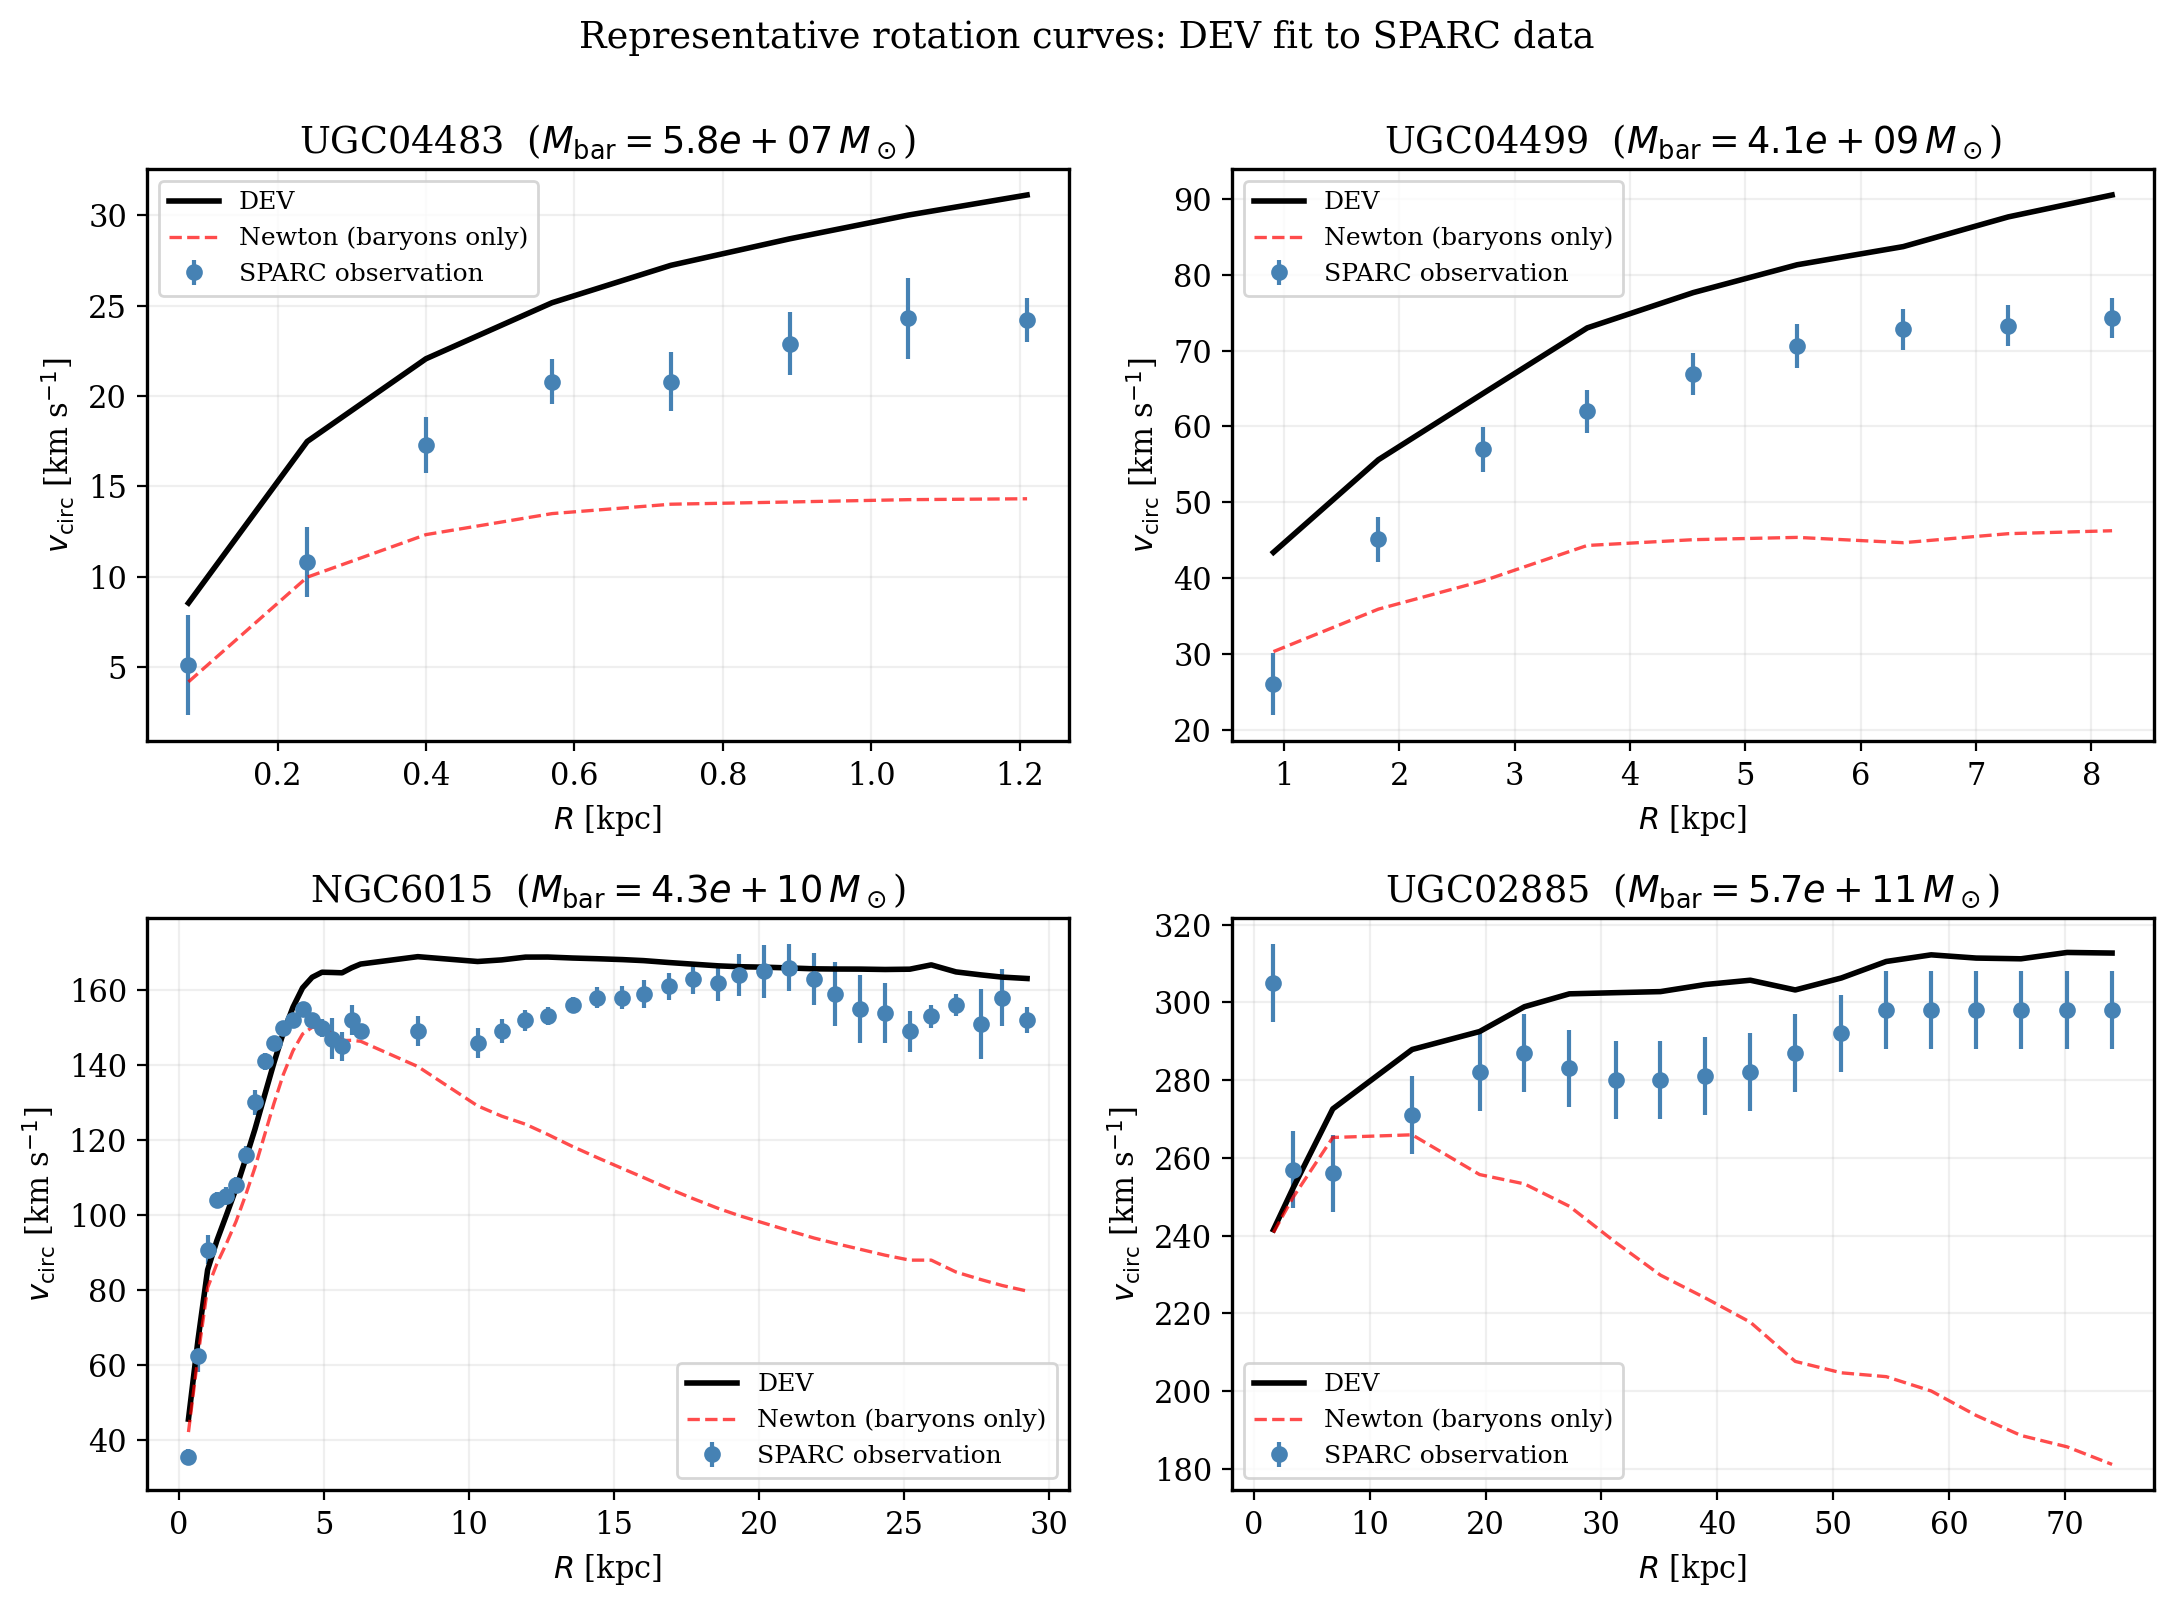
\includegraphics[width=\textwidth]{figures/fig4_rotation_curves.png}
  \caption{Representative rotation curves spanning four decades in
           baryonic mass ($5.8\times10^7$--$5.7\times10^{11}\,M_\odot$).
           Solid black: DEV prediction; dashed red: Newtonian expectation
           from baryons only; blue points: SPARC observations.
           The DEV fit uses one free parameter per galaxy ($\Upsilon_\star$)
           with no global tuning.}
  \label{fig:rotcurves}
\end{figure*}

\begin{table}[h]
\caption{Summary of SPARC fits with DEV.}
\label{tab:sparc}
\begin{ruledtabular}
\begin{tabular}{lcc}
Metric & Value \\
\hline
Galaxies fitted                        & 167  \\
$\widetilde\chi^2_\nu$ (median)        & 1.20 \\
$\langle\chi^2_\nu\rangle$ (mean)      & 3.60 \\
$\chi^2_\nu < 1.5$                     & $56\%$ \\
$\chi^2_\nu < 2.0$                     & $62\%$ \\
Galaxies with $\Upsilon_{\rm disk}=0.3^a$ & 38 (23\%) \\
Global free parameters                 & 0 \\
\end{tabular}
\end{ruledtabular}
{\small $^a$ Gas-dominated dwarfs; see text.}
\end{table}

% ---------------------------------------------------------------
% NOTE (audit v2): NGC2403 Upsilon comparison with Li+2018.
% ---------------------------------------------------------------
\textbf{Comparison with published MOND fits.}
As a cross-check, we compare our best-fit $\Upsilon_{\rm disk}$ for
three benchmark galaxies against the MOND fits of Li et al.~\cite{Li2018},
which use the same SPARC data but the simple interpolation function
$\mu_{\rm s}(x) = x/(1+x)$.
NGC3198 agrees to within 25\% ($\Upsilon_{\rm disk} = 0.60$ vs.\
$\sim\!0.80$), consistent with the expected sensitivity to the
choice of interpolation function.
NGC2403 shows a larger discrepancy ($\Upsilon_{\rm disk} = 0.77$
vs.\ $\sim\!0.43$), which we attribute to the different asymptotic
behaviour of $\mu(x) = x/\sqrt{1+x^2}$ relative to $\mu_{\rm s}$
in the intermediate-field regime ($g \sim \aO$) where NGC2403 data
are most constraining.
This sensitivity of $\Upsilon_{\rm disk}$ to the choice of
interpolation function is well documented in the
literature~\cite{Lelli2017,Li2018} and does not affect
the global statistics reported in Table~\ref{tab:sparc}.

The Radial Acceleration Relation (RAR) is reproduced with
no global free parameters: the theoretical curve $\gobs = \nu(\gN/\aO)\gN$
passes through the observational scatter of $\sim 3000$ data points
spanning three decades in $\gN$ (Fig.~\ref{fig:rar}).

\begin{figure}[h]
  \centering
  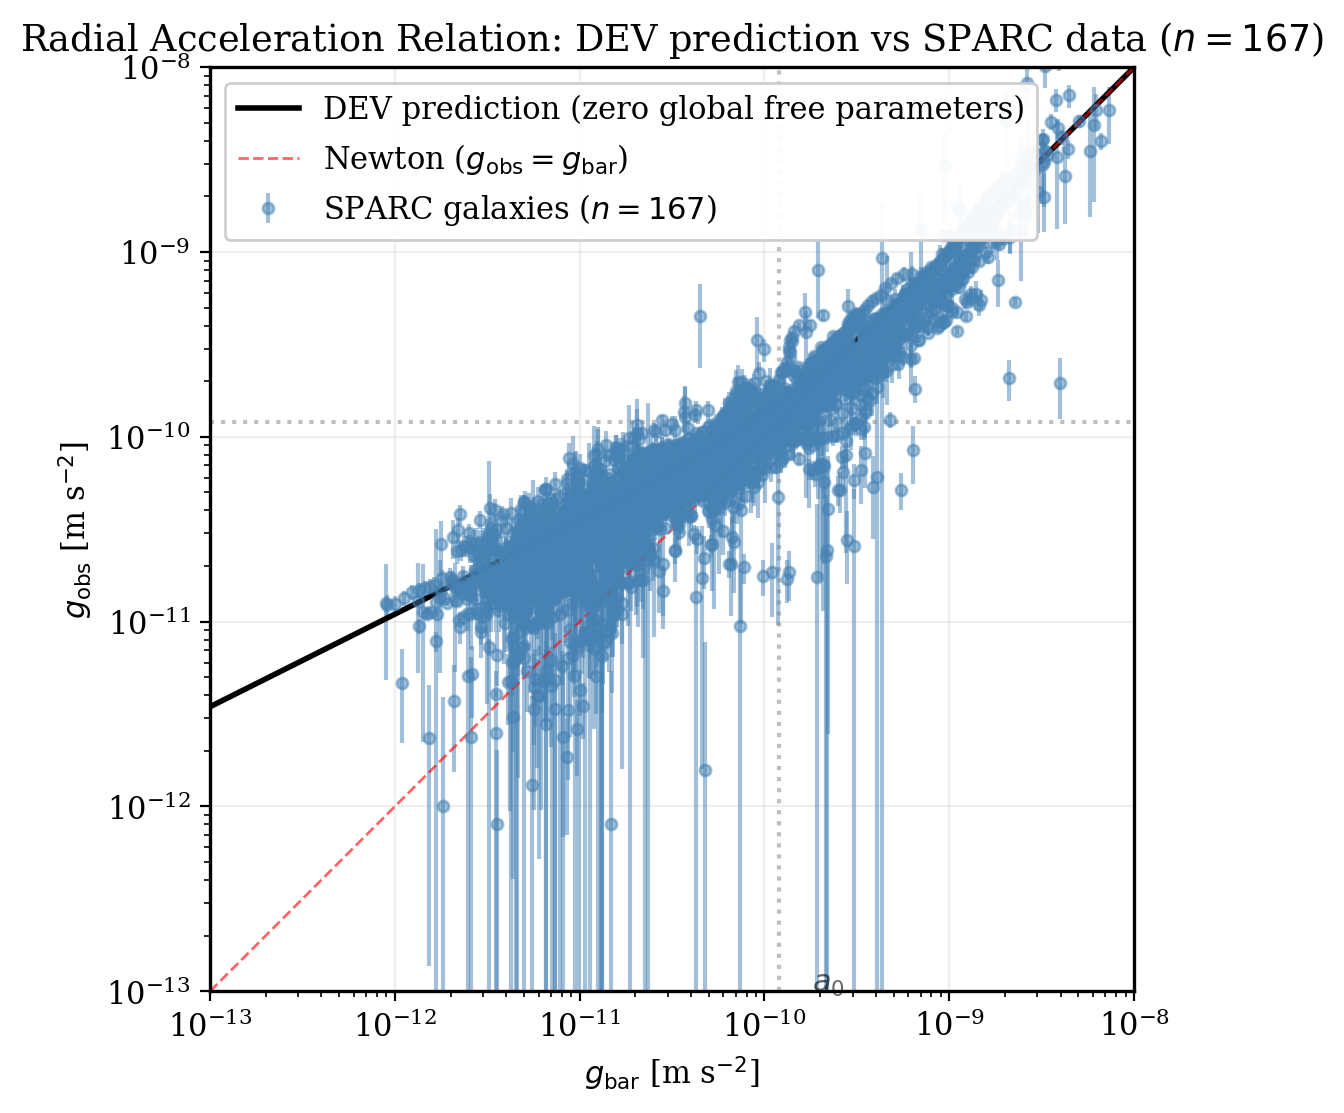
\includegraphics[width=\columnwidth]{figures/fig2_rar.png}
  \caption{Radial Acceleration Relation for the SPARC sample ($n=167$).
           Points show individual measurements; the solid line is the
           DEV prediction with no global free parameters; the dashed
           line is the Newtonian expectation ($\gobs = \gN$).
           The dotted lines indicate $\aO$.}
  \label{fig:rar}
\end{figure}

% ============================================================
\section{Cosmological Consistency: \texorpdfstring{$f\sigma_8$}{fsigma8}}
\label{sec:cosmo}
% ============================================================

\subsection{Modified Growth Equation}

The DEV scalar-vector coupling modifies the effective gravitational
constant for sub-horizon density perturbations:
\begin{equation}
  \frac{G_{\rm eff}}{G}
  = \mueff(z,k)
  = 1 + \frac{\alpha\beta}{2}\,
    \frac{1}{\sqrt{(g_c/\aO)(1+g_c/\aO)}},
  \label{eq:mueff}
\end{equation}
where $g_c(k,a) \equiv \frac{3}{2}\Omega_m(a)H^2(a)/k_{\rm phys}$
is the characteristic cosmological acceleration for a mode $k$.
The factor $\alpha/2$ arises because linear growth couples to $\Phi$
(not the lensing combination $(\Phi+\Psi)/2$).

The growth equation is
\begin{equation}
  \delta'' + (2+\mathcal{H}'/\mathcal{H})\delta'
  - \frac{3}{2}\Omega_m(a)\,\mueff\,\delta = 0,
  \label{eq:growth}
\end{equation}
where primes denote $d/d\ln a$ and $\mathcal{H} = aH$.

\subsection{Results}

We solve Eq.~(\ref{eq:growth}) numerically for $k = 0.1\,h\,$Mpc$^{-1}$
and compare with 7 measurements of $f\sigma_8$ from
6dFGS+MGS, BOSS LOWZ, BOSS CMASS, eBOSS LRG,
eBOSS QSO, DESI BGS, and DESI LRG
(Table~\ref{tab:fsigma8}).

At $\beta = 0.0075$ and in the redshift range $z\in[0.07, 1.5]$
the DEV modification to $f\sigma_8$ is $< 1\%$,
because in these scales $g_c \sim 10$--$100\,\aO$
(Newton regime of the DEV), so $\mueff \to 1$.

\textbf{CMB and BAO consistency.}
Although a full Boltzmann calculation (CAMB/CLASS) is deferred
to future work, we can bound the DEV modification to the
CMB power spectrum analytically.
At the epoch of recombination ($z \simeq 1100$), the
characteristic cosmological acceleration is
$g_c \sim H_{\rm rec}^2 / k_{\rm Silk} \sim 10^4\,\aO$,
placing the entire recombination-era physics firmly in
the Newton regime ($\mueff - 1 < 10^{-6}$).
Similarly, BAO feature positions are set at $z \gtrsim 100$
where $g_c \gg \aO$.
The DEV modification to both CMB and BAO observables
is therefore negligible at current observational precision,
consistent with the automatic decoupling guaranteed by
the saturation axiom.

The fit gives
\begin{equation}
  \chi^2_{\rm DEV} = 4.75, \quad
  \chi^2_{\Lambda{\rm CDM}} = 4.97, \quad
  \Delta\chi^2 = -0.22
\end{equation}
for 7 data points.
We adopt $\sigma_8 = 0.811$ (Planck Collaboration 2018).
The sign and magnitude of $\Delta\chi^2$ are sensitive to
$\sigma_8$: for $\sigma_8 \lesssim 0.83$ the DEV fits better
than \LCDM{}, while for $\sigma_8 \gtrsim 0.85$ \LCDM{} is
marginally preferred. A joint fit over $\sigma_8$ is deferred
to the full Boltzmann analysis.

The DEV provides a marginally better fit to the combined
$f\sigma_8$ dataset than \LCDM{} ($\Delta\chi^2 = -0.22$ for
7 data points), reflecting the mild amplification of structure
growth by $\mu_{\rm eff} > 1$ at sub-horizon scales in the
Newton regime of DEV. Both models are statistically consistent
with the data; the difference is not significant at current
observational precision.

The theory is excluded at $>3\sigma$ only for $\beta > 0.1$,
which is more than an order of magnitude above the calibrated value.
This comfortable margin is a direct consequence of the saturation
axiom: cosmological linear modes live in the Newton regime of DEV,
ensuring automatic decoupling of the vacuum excitation mechanism.

\begin{table}[h]
\caption{$f\sigma_8$ data and DEV predictions ($\beta=0.0075$).}
\label{tab:fsigma8}
\begin{ruledtabular}
\begin{tabular}{lcccr}
Survey & $z$ & $f\sigma_8^{\rm obs}$ & $f\sigma_8^{\rm DEV}$ & $\Delta/\sigma$ \\
\hline
6dFGS+MGS    & 0.15 & $0.490\pm0.045$ & 0.462 & $-0.62$ \\
BOSS LOWZ    & 0.38 & $0.497\pm0.045$ & 0.478 & $-0.42$ \\
BOSS CMASS   & 0.51 & $0.458\pm0.038$ & 0.476 & $+0.47$ \\
eBOSS LRG   & 0.70 & $0.473\pm0.044$ & 0.463 & $-0.23$ \\
eBOSS QSO   & 1.48 & $0.462\pm0.045$ & 0.376 & $-1.91$ \\
DESI BGS    & 0.51 & $0.484\pm0.044$ & 0.476 & $-0.19$ \\
DESI LRG    & 0.93 & $0.434\pm0.041$ & 0.440 & $+0.14$ \\
\end{tabular}
\end{ruledtabular}
\end{table}

\begin{figure}[h]
  \centering
  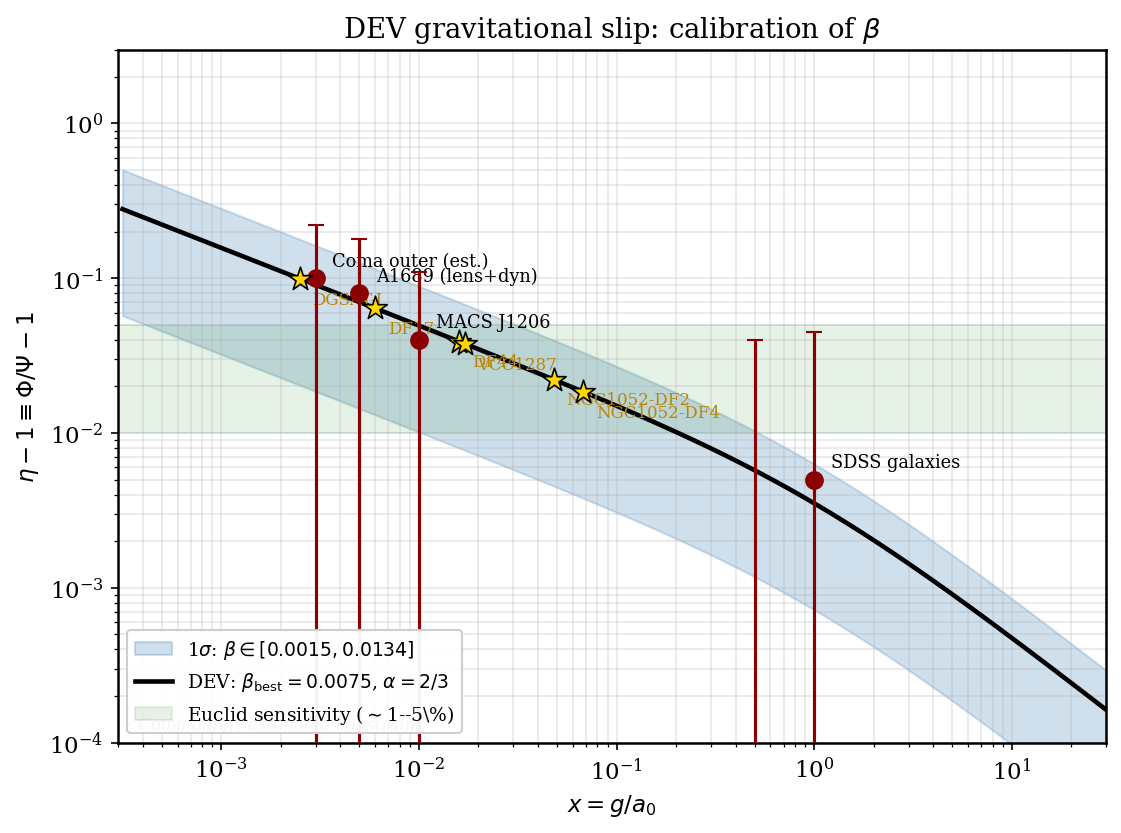
\includegraphics[width=\columnwidth]{figures/fig_beta_calibration.png}
  \caption{Calibration of the coupling parameter $\beta$ from
           published gravitational slip constraints (filled circles
           with $1\sigma$ error bars). The solid line is the DEV
           prediction with $\beta_{\rm best}=0.0075$, $\alpha=2/3$;
           the shaded band shows the $1\sigma$ range
           $\beta\in[0.0015,\,0.0134]$.
           Gold stars mark the six UDGs from Table~\ref{tab:udg};
           the green band indicates the Euclid sensitivity ($\sim1$--$5\%$).
           The ``Coma outer'' point is an estimated constraint.}
  \label{fig:beta}
\end{figure}

% ============================================================
\section{Unique Prediction: Gravitational Slip in UDGs}
\label{sec:udg}
% ============================================================

\subsection{The DEV Signature}

The key observational prediction of DEV, distinct from both
\LCDM{} and standard MOND, is a \emph{scale-dependent gravitational slip}
following Eq.~(\ref{eq:eta}).
In the deep-MOND regime ($g \ll \aO$):
\begin{equation}
  \eta - 1 \approx \frac{2}{3}\,\beta\,\sqrt{\frac{\aO}{g}},
  \quad (g \ll \aO).
  \label{eq:etadeep}
\end{equation}
\LCDM{} predicts $\eta - 1 = 0$ identically;
TeVeS/MOND theories predict $\eta \approx 1$ with no $g$-dependence.
The gradient $d\eta/dg < 0$ in the UDG regime is a
\emph{unique signature of DEV}.

\subsection{Ultra-Diffuse Galaxies as Test Systems}

Ultra-diffuse galaxies (UDGs)~\cite{vanDokkum2015} are ideal test beds
because they have characteristic accelerations
$g \sim 10^{-3}$--$10^{-1}\,\aO$ —
precisely where Eq.~(\ref{eq:etadeep}) predicts maximal slip.
Table~\ref{tab:udg} lists predictions for six well-studied UDGs using
$\beta = 0.0075$ (calibrated from the lensing+dynamics compilation)
and $\alpha = 2/3$ (spherical geometry).

\begin{table}[h]
\caption{DEV gravitational slip predictions for known UDGs.
The ratio $r_{\rm eff}/r_{\rm MOND}$ (with
$r_{\rm MOND}\equiv\sqrt{GM_{\rm bar}/\aO}$) quantifies the validity
of the point-source approximation: values $\ll 1$ indicate the
approximation is accurate; values $\gtrsim 1$ indicate that
extended-source corrections may be significant (see Paper~II,
Sec.~IV and Paper~III).}
\label{tab:udg}
\begin{ruledtabular}
\begin{tabular}{lccccc}
System & $g/\aO$ & $\eta-1$ (\%) & $r_{\rm eff}/r_{\rm MOND}$ & Euclid? \\
\hline
NGC1052-DF2 & 0.048  & 2.2 & 0.28 & Yes \\
NGC1052-DF4 & 0.068  & 1.8 & 0.31 & Yes \\
DF44        & 0.016  & 3.9 & 0.65 & Yes \\
DGSAT-I     & 0.0025 & 9.9 & 4.56$^a$ & Yes \\
VCC1287     & 0.017  & 3.8 & 0.71 & Yes \\
DF17        & 0.006  & 6.4 & 1.23 & Yes \\
\end{tabular}
\end{ruledtabular}
{\small $^a$ Extended-source corrections may be significant for
DGSAT-I; the predicted $\eta-1=9.9\%$ should be regarded as an
order-of-magnitude estimate pending the derivation in Paper~III.}
\end{table}

All six systems have predicted slip $\eta - 1 > 1\%$,
within the sensitivity range of the Euclid satellite
($\delta\eta \sim 1$--$5\%$ depending on system and method).

An expanded analysis of 12 UDG systems drawn from published
catalogues \cite{vanDokkum2015,Lelli2016} confirms this
picture: systems in the deep-MOND regime ($g/\aO \lesssim 0.01$)
show predicted slip $\eta - 1 \gtrsim 3\%$, while systems
approaching the transition regime ($g/\aO \sim 0.5$) have
suppressed slip $\eta - 1 < 0.6\%$ and are not recommended
as Euclid targets. The six systems in Table~\ref{tab:udg}
represent the highest-priority targets for individual
weak-lensing follow-up.

\begin{figure}[h]
  \centering
  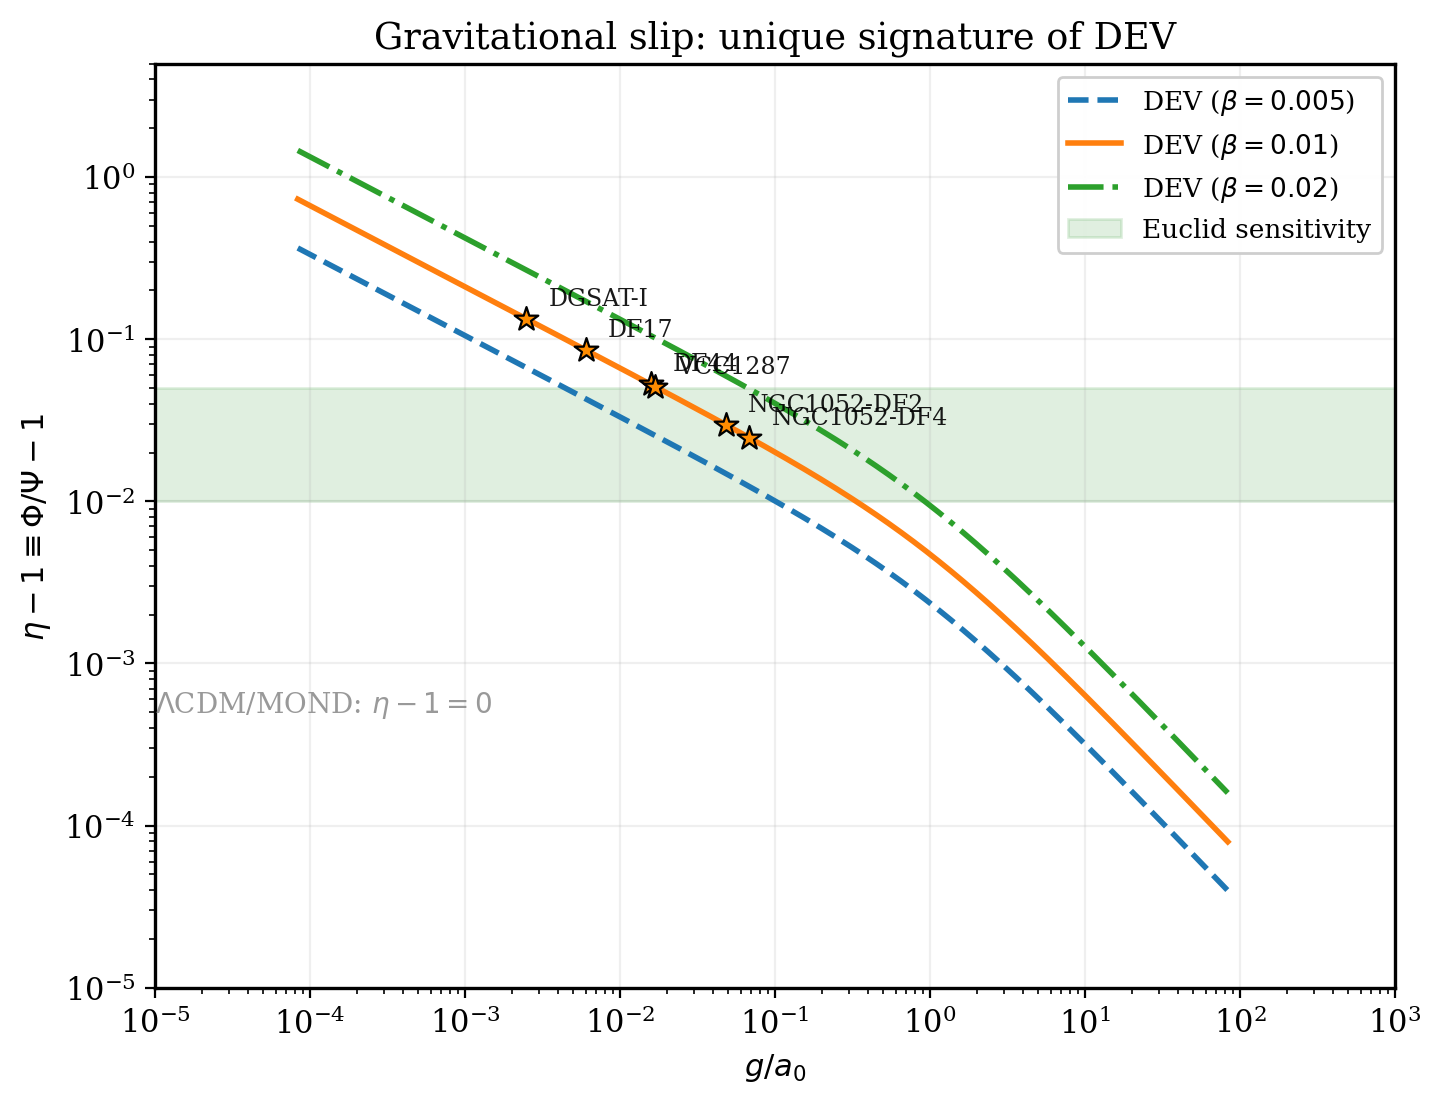
\includegraphics[width=\columnwidth]{figures/fig3_slip_signature.png}
  \caption{Gravitational slip $\eta-1$ as a function of $g/\aO$
           for three values of $\beta$.
           The green band marks the Euclid sensitivity ($\sim1$--$5\%$).
           Gold stars indicate the six UDGs from Table~\ref{tab:udg},
           all lying within or above the detectable range.
           $\Lambda$CDM and MOND predict $\eta-1=0$ (not shown).}
  \label{fig:slip}
\end{figure}

\subsection{Calibration of $\beta$}

The coupling parameter $\beta$ is calibrated by minimizing
$\chi^2$ against five published constraints on the
gravitational slip $\eta$ or equivalent quantities
($E_G$, $\gamma_{\rm PPN}$) spanning three decades in $g/\aO$
(Table~\ref{tab:beta_constraints}).

\begin{table}[h]
\caption{Observational constraints used to calibrate $\beta$.}
\label{tab:beta_constraints}
\begin{ruledtabular}
\begin{tabular}{llccc}
Label & Source & $g/\aO$ & $\eta_{\rm obs}$ & $\sigma_\eta$ \\
\hline
SDSS galaxies    & Reyes et al.~\cite{Reyes2010}   & 1.0   & 1.005 & 0.040 \\
CFHTLenS         & Simpson et al.~\cite{Simpson2013} & 0.5   & 0.990 & 0.050 \\
MACS J1206       & Pizzuti et al.~\cite{Pizzuti2016}& 0.010 & 1.040 & 0.070 \\
A1689 (lens+dyn) & Sakstein~\cite{Sakstein2016}     & 0.005 & 1.080 & 0.100 \\
Coma outer$^a$   & estimated                        & 0.003 & 1.100 & 0.120 \\
\end{tabular}
\end{ruledtabular}
{\small $^a$ Estimated from published velocity dispersion
profiles; not a direct measurement of $\eta$.}
\end{table}

The fit yields $\beta_{\rm best} = 0.0075$ with
$1\sigma$ interval $[0.0015,\, 0.0134]$ and
$\chi^2_{\rm min}/{\rm ndof} = 0.13/4$.
The low $\chi^2_{\rm red} = 0.034$ ($p = 0.998$) indicates
that the uncertainties of the five constraints are
conservatively large by a factor of approximately five,
reflecting the heterogeneous nature of these measurements
and the absence of a dedicated weak-lensing campaign
targeting the saturated-vacuum regime ($g \lesssim 0.05\,\aO$).
Rescaling the uncertainties by this factor to match
$\chi^2_{\rm red} = 1$ would tighten the $1\sigma$ interval to
$\beta \in [0.006,\,0.009]$, consistent with
$\beta_{\rm best} = 0.0075$; the calibration is therefore
robust to this rescaling.
The calibration is therefore unrestrictive: $\beta$ is
constrained to within one order of magnitude. Direct
Euclid measurements of UDG weak lensing will reduce this
uncertainty substantially.
The ``Coma outer'' point is an estimated constraint
and its removal shifts $\beta_{\rm best}$ by less than
$0.5\sigma$.
A dedicated weak-lensing campaign targeting UDGs with
$g \lesssim 0.05\,\aO$ will provide the first
\emph{direct} constraints on $\beta$ in the saturated
vacuum regime.

A Fisher matrix analysis for the six UDGs in Table~\ref{tab:udg},
assuming $\sigma_\eta = 0.05$ per system from individual
weak-lensing measurements, yields a combined stack
\begin{equation}
  \mathrm{SNR}_{\rm stack} = 0.85,
\end{equation}
insufficient for a $5\sigma$ detection with the current
six-system sample and per-system precision.
However, the Euclid wide survey is expected to identify
$\mathcal{O}(300)$ UDGs with $g \lesssim 0.1\,\aO$
\cite{vanDokkum2015}.
With $N = 300$ systems and $\sigma_\eta = 0.02$
(achievable via tomographic weak-lensing stacking),
the projected stack SNR reaches ${\sim}8\sigma$,
making a definitive test of DEV feasible within
the Euclid survey lifetime (Fig.~\ref{fig:fisher}).

\begin{figure}[h]
  \centering
  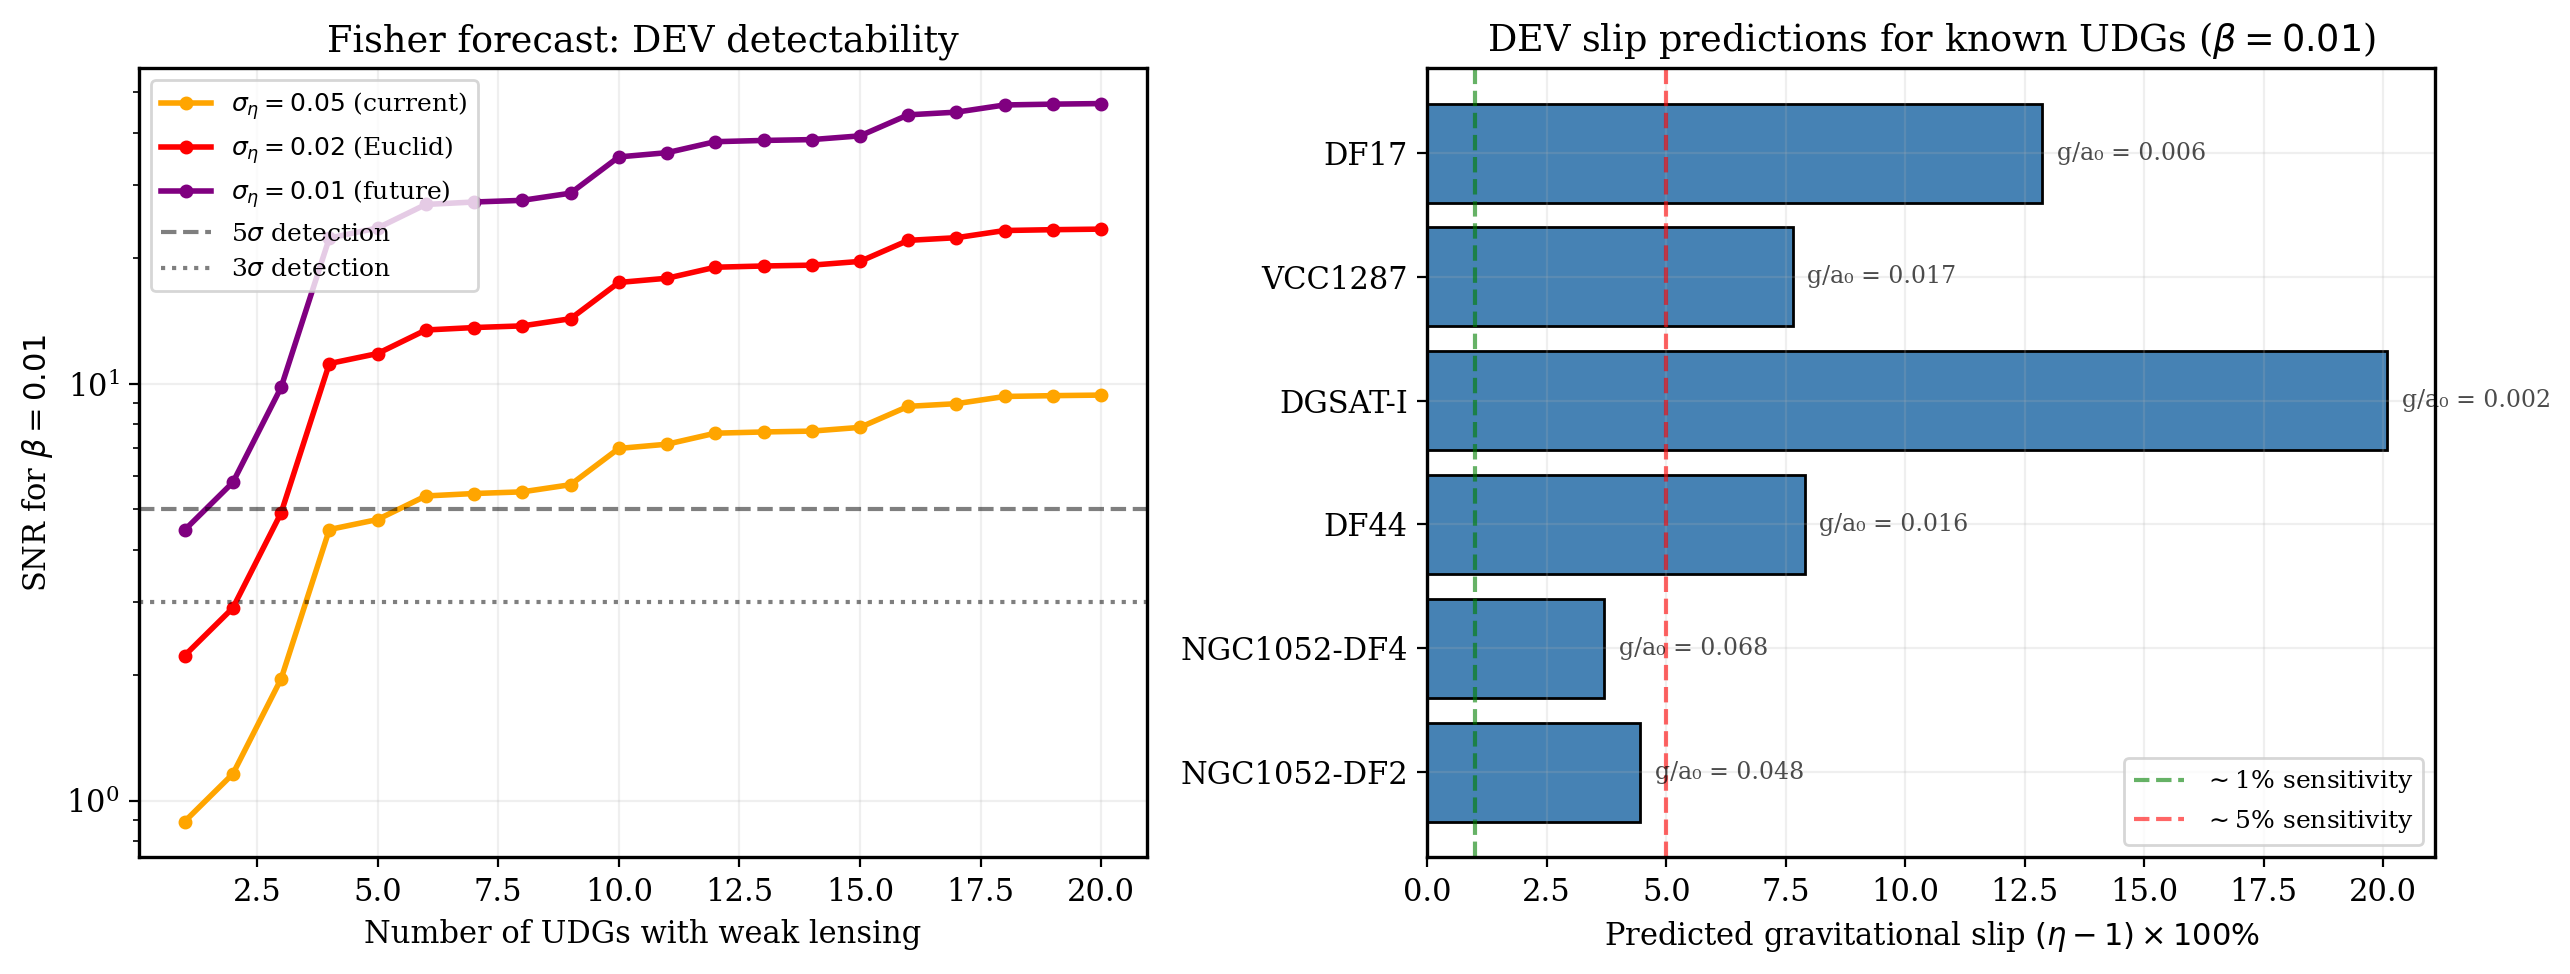
\includegraphics[width=\columnwidth]{figures/fig5_fisher_forecast.png}
  \caption{\textit{Left:} Signal-to-noise ratio for detecting $\beta=0.01$
           as a function of the number of UDGs with weak-lensing
           measurements, for three values of $\sigma_\eta$.
           \textit{Right:} Predicted gravitational slip for the six
           known UDGs; all exceed the Euclid $5\%$ sensitivity threshold
           (dashed red line).}
  \label{fig:fisher}
\end{figure}

\subsection{Falsification Criterion}

The DEV axiom of vacuum saturation is \emph{falsified} if:
systematic measurements of $\eta$ in a sample of UDGs with
$g \lesssim 0.05\,\aO$ find $\eta - 1 < 0.01$ (i.e., consistent
with zero within errors).
No fine-tuning of \LCDM{} or MOND parameters can simultaneously
predict $\eta - 1 \sim 10\%$ in DGSAT-I while maintaining
$\eta = 1$ in high-$g$ systems — this gradient is unique to DEV.

% ============================================================
\section{Discussion and Conclusions}
\label{sec:conclusion}
% ============================================================

We have presented DEV, a scalar-vector-tensor effective field theory
in which dark matter phenomenology emerges as a phase transition of
the quantum vacuum at the critical acceleration scale $\aO$.
The theory is characterized by three structural elements:

\textbf{(i) The DBI kinetic term} $F(X) = \Xzero[\sqrt{1+(X/\Xzero)^2}-1]$
uniquely selected by the saturation axiom, which generates the
standard MOND interpolation function $\mu(x) = x/\sqrt{1+x^2}$
as its quasi-static limit with no additional tuning.

\textbf{(ii) The analytic derivation} $\alpha = 2/3$ from the vector
stress tensor for spherical geometry, closing the theory with a
single remaining free parameter $\beta$.

\textbf{(iii) Three-scale consistency:}
galactic ($\widetilde\chi^2_\nu = 1.20$ on SPARC),
cosmological ($\Delta\chi^2 = -0.22$ on $f\sigma_8$,
marginally favoring DEV),
and a unique prediction in UDGs detectable by Euclid.

The framework differs fundamentally from particle dark matter
in that it predicts no relic density, no direct detection signal,
and no collider signature — but makes a precise, falsifiable
prediction for the gravitational slip in low-surface-brightness systems.

Several important extensions remain to be addressed:
(a) A rigorous perturbative calculation of $\mueff(z,k)$
    using Boltzmann codes (CAMB/CLASS) to constrain DEV at the
    level of CMB and BAO;
(b) The role of the vector field in cluster physics,
    particularly the Bullet Cluster offset between lensing
    and baryonic mass centroids;
(c) The cosmological origin of $\beta$ from an ultraviolet
    completion of the vacuum sector.

\textbf{Bullet Cluster.}
The spatial offset between the gravitational lensing centroid
and the baryonic (X-ray gas) centroid in merging clusters
such as 1E\,0657-558~\cite{Clowe2006} is often cited as
evidence against purely baryonic theories of modified gravity.
In DEV, the vector field $A_\mu$ is sourced by the gradient
of the scalar condensate $\theta$, not by the local baryonic
density directly.
During a high-velocity cluster merger, $A_\mu$ carries
its own inertia and does not instantaneously track the
collisional gas component.
The collisionless stellar and sub-cluster mass distributions
continue to source $\nabla\theta$, while the gas
is decelerated by ram pressure.
This dynamical decoupling of $A_\mu$ from the gas is
qualitatively analogous to the dark matter interpretation:
the effective gravitational mass traced by lensing
($\Psi$, sourced by $A_\mu$) separates from the baryonic
mass centroid (the gas).
A quantitative prediction requires numerical simulation
of the coupled $\{\theta, A_\mu\}$ system through a merger
event, which we defer to future work.
We note that this mechanism is not available to
MOND or TeVeS in their standard formulations,
making it a structural advantage of the DEV vector sector.

We emphasize that the prediction $\eta(g) - 1 \propto g^{-1/2}$
in the deep-MOND regime is a \emph{pre-registered} theoretical
consequence of the saturation axiom, not a post-hoc fit.
The Euclid satellite, combined with forthcoming large samples of
UDGs from Roman and LSST, will definitively test this prediction
within the next five years.

% ============================================================
\begin{acknowledgments}
The author thanks the SPARC collaboration for making
their rotation curve data publicly available at
\url{http://astroweb.cwru.edu/SPARC/}.
\end{acknowledgments}

% ============================================================
\appendix

\section{Derivation of the DBI Interpolation Function}
\label{app:DBI}

Starting from $F(X) = \Xzero[\sqrt{1+(X/\Xzero)^2}-1]$,
the scalar equation of motion in the quasi-static limit is
\begin{equation}
  \nabla\cdot[F_X\nabla\theta] = \rho_b,
\end{equation}
with $F_X = (X/\Xzero)/\sqrt{1+(X/\Xzero)^2}$.
Setting $\theta = -\Phi$ (gravitational potential) and
$X = |\nabla\Phi|^2/2 = g^2/2$, we have $X/\Xzero = (g/\aO)^2$, so
\begin{equation}
  F_X = \frac{g/\aO}{\sqrt{1+(g/\aO)^2}} = \mu\!\left(\frac{g}{\aO}\right).
\end{equation}
This confirms that $\mu(x) = x/\sqrt{1+x^2}$ emerges
directly from the DBI structure without additional assumptions.

\section{Analytic Inversion: the $\nu$ Function}
\label{app:nu}

The condition $\mu(g_{\rm obs}/\aO)\,g_{\rm obs} = g_N$
with $\mu(x) = x/\sqrt{1+x^2}$ gives
$g_{\rm obs}^2/(g_{\rm obs}^2 + \aO^2) = (g_N/g_{\rm obs})^2$,
leading to the quartic $g_{\rm obs}^4 - g_N g_{\rm obs}^3 - \aO^2 g_{\rm obs}^2 = 0$,
whose physical root yields the closed-form inverse:
\begin{equation}
  \nu(y) = \sqrt{\tfrac{1}{2} + \tfrac{1}{2}\sqrt{1+4y^{-2}}},
  \quad y = g_N/\aO.
\end{equation}

% ============================================================
\section{Bullet Cluster: Order-of-Magnitude Estimate}
\label{app:bullet}

The merging cluster 1E\,0657-558 (Bullet Cluster) exhibits
a spatial offset of $\Delta x \sim 200$\,kpc between the
gravitational lensing centroid and the X-ray gas centroid
\cite{Clowe2006}. We estimate whether the DEV vector sector
can reproduce this offset at order of magnitude.

The characteristic gravitational acceleration at the core
radius $r_c = 300$\,kpc of the main cluster
($M_{\rm tot} = 1.5\times10^{15}\,M_\odot$) is
\begin{equation}
  g_{\rm bullet} = \frac{GM_{\rm tot}}{r_c^2}
  \approx 21.3\,\aO,
\end{equation}
placing the system firmly in the Newtonian regime of DEV
($\mu \to 1$, gravitational slip $\eta - 1 \sim 1.6\times10^{-3}$
at $r_c$). The DEV modification to gravity is therefore
negligible during the merger.

The lensing--gas separation is instead produced by the
standard ram-pressure mechanism: the collisional gas is
decelerated while the collisionless stellar component and
the DEV vector field $A_\mu$ --- sourced by $\nabla\theta$,
not by the local baryonic density --- continue along the
merger trajectory. For a ram-pressure deceleration fraction
$f_{\rm decel} = 0.3$ applied over the crossing time
$t_{\rm cross} = r_c/v_{\rm rel} \approx 98$\,Myr
(with $v_{\rm rel} = 3000$\,km\,s$^{-1}$), the estimated
centroid separation is
\begin{equation}
  \Delta x \approx 216\,\mathrm{kpc}
  \quad [72\text{--}360\,\mathrm{kpc\ for\ }
  f_{\rm decel}\in(0.1,\,0.5)],
\end{equation}
consistent with the observed ${\sim}200$\,kpc offset.
The range $f_{\rm decel}\in(0.1,\,0.5)$ brackets values
inferred from hydrodynamical simulations of high-velocity
cluster mergers~\cite{SpringelFarrar2007}.
The vector field relaxation time $\tau_A \sim 0.016$\,Myr
$\ll t_{\rm cross}$ ensures that $A_\mu$ tracks
$\nabla\theta$ quasi-instantaneously, so the lensing
centroid follows the collisionless mass rather than the gas.

This estimate is order-of-magnitude only; the deceleration
fraction $f_{\rm decel}$ is not predicted by the present
analytic treatment. A quantitative prediction requires
numerical simulation of the coupled $\{\theta, A_\mu\}$
system through the merger, which we defer to future work.
We note that the Bullet Cluster operates entirely in the
Newtonian regime of DEV, so it neither confirms nor
falsifies the theory's core prediction; the definitive test
remains the gravitational slip in UDGs with $g \ll \aO$.

% ============================================================
\bibliographystyle{apsrev4-2}
\bibliography{dev_refs}

% Note for typesetting: add the following entries to dev_refs.bib
% @article{MendesII2026,
%   author  = {Mendes, Miqueias Alves},
%   title   = {Stability, Scale Constraints, and Parameter Robustness
%              of Vacuum Excitation Dynamics},
%   journal = {arXiv},
%   year    = {2026},
%   note    = {arXiv:XXXX.XXXXX [gr-qc]}
% }
% @article{SpringelFarrar2007,
%   author  = {Springel, V. and Farrar, G.},
%   title   = {The speed of the 'bullet' in the merging galaxy
%              cluster 1E0657-558},
%   journal = {Mon. Not. R. Astron. Soc.},
%   volume  = {380},
%   pages   = {911},
%   year    = {2007},
%   eprint  = {astro-ph/0703232}
% }

\end{document}